\documentclass[12pt, a4paper]{report}
\usepackage[utf8]{inputenc}
\usepackage[italian]{babel}
\usepackage{float}
\usepackage{graphicx}
\usepackage{newlfont}
\usepackage{hyperref}
\usepackage{multirow}
\usepackage{subfiles}
\usepackage{listings}
\usepackage{multicol}
\usepackage{dsfont}
\usepackage[toc,page]{appendix}
\usepackage{proof}
\usepackage{wrapfig}
\usepackage{amsmath,amssymb,amsthm,textcomp}

\usepackage{listings, xcolor}
\lstset{
tabsize = 1, %% set tab space width
showstringspaces = false, %% prevent space marking in strings, string is defined as the text that is generally printed directly to the console
numbers = left, %% display line numbers on the left
commentstyle = \color{green}, %% set comment color
keywordstyle = \color{blue}, %% set keyword color
stringstyle = \color{red}, %% set string color
rulecolor = \color{black}, %% set frame color to avoid being affected by text color
basicstyle = \small \ttfamily , %% set listing font and size
breaklines = true, %% enable line breaking
numberstyle = \tiny,
}


\title{Report Progetto Compilatori ed Interpreti}
\author{Marco Benito Tomasone 1038815\\
Luca Genova 1038843\\
Simone  Boldrini 1038792}
\date{2021-2022}

\begin{document}
    \maketitle
    \tableofcontents
    \chapter{Introduzione}
    Questo documento è il Report per il progetto del corso di  Compilatori ed Interpreti del prof. Cosimo Laneve A.S. 2021/2022. Il progetto ha come obiettivo quello di costruire un compilatore per il linguaggio \emph{AssetLan}.
    AssetLan è un semplice linguaggio imperativo con asset, in cui i parametri possono  essere sia standard che asset, con ricorsione e senza mutua ricorsione. 
    \section{Grammatica del Linguaggio}
    Ogni programma in AssetLan è formato da quattro parti principali che sono le dichiarazioni di variabili, le dichiarazioni degli asset, le dichiarazioni delle funzioni e la chiamata a delle funzioni. I tipi permessi per le variabili sono  \emph{int} e \emph{bool}, mentre per le funzioni oltre ai due tipi sopracitati è permesso dichiarare funzioni \emph{void}. I parametri asset hanno tipo \emph{asset}. 

    Nella dichiarazione di funzioni oltre al tipo e al nome della funzione bisogna indicare una lista di parametri tra parentesi tonde e una lista di asset tra parentesi quadre. Nel corpo di una funzione è possibile fare molteplici dichiarazioni di variabili e poi definire degli statement. 
    Uno statement può essere un assegnamento, una funzione move che permette di spostare il contenuto di un asset all'interno di un altro asset (svuotando il primo asset), una print, una transfer, una return, un \emph{if-then-else} oppure una chiamata a funzione. 
    Rispetto alla grammatica che ci è stata fornita inizialmente abbiamo apportato due piccole modifiche: 
    \begin{lstlisting}      
function: (type | 'void') ID '('(decp)?')' '['(adec)?']' {' (dec';')* statement* '}' ;
decp: dec;
    \end{lstlisting}  
    La prima è per separare la dichiarazione dei parametri formali di una funzione dalle dichiarazioni delle variabili nel corpo della funzione. Per fare ciò è stato inserito un nuovo simbolo non terminale \emph{decp} che richiama il non terminale \emph{dec}.
    \begin{lstlisting}      
initcall: ID '(' (exp (',' exp)* )? ')' '[' (bexp (',' bexp)* )? ']' ;
bexp: exp  ;
    \end{lstlisting}
La seconda modifica apportata riguarda l'introduzione di un nuovo simbolo \emph{bexp} che sostituisce le chiamate al simbolo exp all'interno dei parametri asset nella chiamata di una funzione. 
    \chapter{Analisi Lessicale e Sintattica}
    Le prime due fasi del compilatore per il linguaggio AssetLan hanno previsto la costruzione dell'analizzatore lessicale e sintattico. 
    \emph{L'analizzatore lessicale} prende in input le stringhe di codice in AssetLan e ritorna una lista di token. L'analizzatore lessicale genera degli errori dal momento in cui non riconosce un certo token all'interno della grammatica. \\
    \emph{L'analizzatore sintattico (parser)} prende in input la lista di token generati dall'analizzatore lessicale e cerca di ricostruire l'Albero di Sintassi Astratta (AST). Se la lista di token non rispetta la grammatica, non sarà possibile costruire l'albero ed il parser genererà un errore. \\
    Per la costruzione del lexer e del parser abbiamo utilizzato ANTLR, un generatore di parser che utilizza il sistema di parsing LL.\\
    Per ritornare la lista degli errori lessicali e sintattici abbiamo creato la classe \emph{SyntaxErrorListener} che estende la classe \emph{BaseErrorListener}. La classe contiene un ArrayList che conterrà tutti gli errori. Nella funzione \emph{syntaxError}, di cui mostriamo uno snippet di codice in basso, gli errori vengono classificati in lessicali e sintattici in base al riconoscitore che li ha generati (lexer o parser) e verranno poi stampati in un file tramite un \emph{PrintWriter}. 
    \begin{lstlisting}[language = Java , frame = trBL , firstnumber = last , escapeinside={(*@}{@*)}]

public void syntaxError(...){
...
    while(errors.hasNext()) {
        SyntaxError i = (SyntaxError)errors.next();
        if(i.getRecognizer().getClass().getSimpleName().equals("AssetLanLexer"))
            lexicalErrors += "Error: " + i.getMsg() + " at line " + i.getLine() + "\n";
        else
            syntaxErrors += "Error: " + i.getMsg() + " at line " + i.getLine() + "\n";
    }
...
}
    \end{lstlisting} 
    Nel main del nostro compilatore, inziamo leggendo il file in input da compilare nella variabile \emph{charStreams}. Inizializzeremo poi un lexer al quale passeremo il file in input e ci darà in output una lista di token. Questa lista di token verrà data in pasto al parser. Inizializzeremo poi un \emph{errorListener} di tipo \emph{SyntaxErrorListener} precedentemente descritto e lo aggiungeremo come ErrorListener sia al lexer che al parser. Non è necessario rimuovere gli altri errorListener poichè come indicato dalla documentazione di ANTLR è possibile  avere più di un tipo di ErrorListener per queste due classi. 
    \begin{lstlisting}[language = Java , frame = trBL , firstnumber = last , escapeinside={(*@}{@*)}]
        CharStream charStreams = CharStreams.fromFileName(fileName);
        AssetLanLexer lexer = new AssetLanLexer(charStreams);
        CommonTokenStream tokens = new CommonTokenStream(lexer);
        AssetLanParser parser = new AssetLanParser(tokens);

        SyntaxErrorListener errorListener = new SyntaxErrorListener();
        lexer.addErrorListener(errorListener);
        parser.addErrorListener(errorListener);
    \end{lstlisting}
    \section{Esempi}
    In questo primo esempio abbiamo inserito dei token non ammessi dalla grammatica (\$,@,\~, ?). Notiamo come negli errori lessicali siano riportati i primi tre simboli mentre non figura il "?" poichè inserito all'interno di un commento. . 
    \begin{lstlisting}
        asset x;$
        void f(int n)[asset $u, asset v]{
        if (n == 0) {u -o x ;}
        else { u -o x ; v -o x ;}
        }
        void main()[asset a]{
        f(0)[a,a] ;        // semantica di f()[a,a] ?
        transfer @x ;
        }
        main(~)[1] ;
    \end{lstlisting}
   \begin{lstlisting}
        --------LEXICAL ERRORS----------
        Error: token recognition error at: '$' at line 1
        Error: token recognition error at: '$' at line 2
        Error: token recognition error at: '@' at line 8
        Error: token recognition error at: '~' at line 10

        --------SYNTAX ERRORS----------
       \end{lstlisting}
   In questo secondo esempio non abbiamo inserito errori lessicali ma abbiamo inserito le dichiarazioni degli asset e delle variabili dopo le dichiarazioni delle funzioni. Notiamo come dia come errore lessicale la presenza della parola \emph{asset} alla riga 10, mentre si aspetta di trovare una dichiarazione di funzione o un id per richiamare una funzione.
   
    \begin{lstlisting}
        void f()[asset u ,asset v]{
            u -o y ;
            v -o x ;
        }
        void main()[asset u ,asset v]{
            u -o x ;
            u -o y ;
        f()[x,y] ;
        }
        asset x, y ;
        int a,b = 3;
        main()[2,3]
    \end{lstlisting}
    
    \begin{lstlisting}
        --------LEXICAL ERRORS----------

        --------SYNTAX ERRORS----------
        Error: extraneous input 'asset' expecting {'void', 'int', 'bool', ID} at line 10
        Error: mismatched input ',' expecting '(' at line 10
       \end{lstlisting}
   In questo terzo esempio manca il non terminale \emph{initcall} della grammatica, che è obbligatorio. Il parser in questo caso genera un errore dichiando come riconosce l'$<$EOF$>$ invece di trovare un'ulteriore dichiarazione a funzione o la chiamata ad una funzione.
    \begin{lstlisting}
        int a ; 
        asset x ;
        void f(int n)[asset u, asset v, asset w]{
            u -o x ;
            f(n - 1)[v,w,u] ;
        }
        void main()[asset a, asset b, asset c]{
            f(1)[a,b,c] ;
            transfer x ;
        }
    \end{lstlisting}
       \begin{lstlisting}
        --------LEXICAL ERRORS----------

        --------SYNTAX ERRORS----------
        Error: mismatched input ';' expecting '[' at line 5
        Error: extraneous input '<EOF>' expecting {'void', 'int', 'bool', ID} at line 10
       \end{lstlisting}    
 \chapter{Analisi Semantica}
 \section{Environment}
 In questo progetto l’ambiente viene definito come un insieme di scope, gestiti dalla classe \emph{Environment}, che contiene la symbolTable implementata come una lista di HashMap di stringhe e STentry. La classe Environment inoltre contiene un campo \emph{nestingLevel} ed un campo \emph{offset} che servirà come ``contatore" per la gestione dell'offset delle varie variabili. I metodi della classe Environment si occupano della gestione della symbolTable. Ogni volta che si entra in un nuovo ambiente viene creata una nuova symbolTable che viene aggiunta in testa alla lista e viene aumentato il nestingLevel. Allo stesso modo quando si esce da un ambiente viene eliminata la hash map che si trova in testa e diminuito il nestingLevel e ristabilito l'offset. In questa classe sono anche presenti alcune funzioni per lavorare con gli environment:
 \begin{itemize}
    \item \emph{lookup()}: restituisce la entry di un id all'interno della symbolTable
    \item \emph{addDeclaration()}: aggiunge una dichiarazione per un certo id
    \item \emph{exitScope()}: performa l'uscita da uno scope
    \item \emph{newScope()}: performa la creazione di un nuovo scope
    \item \emph{clone()}: crea una nuova instanza di un ambiente a partire da un altro  
    \item \emph{equals()}: restituisce true o false a seconda che due ambienti siano uguali o meno 
 \end{itemize}

 \section{STentry}
 STEntry è un'interfaccia che viene implementata da tre possibili classi che sono:
 \begin{itemize}
    \item \emph{STentryFun}: crea l'istanza dell'STentry di una funzione. Contiene un nodo funzione, il nestingLevel e l'offset.
    \item \emph{STentryVar}: crea l'istanza dell'STentry di una variabile booleana o intera. Contiene il tipo, il nestingLevel e l'offset.
    \item \emph{STentryAsset}: è un'estensione di STentryVar, alla quale aggiunge il campo \emph{liquidity}.
 \end{itemize}

 \section{Check Semantics}
 Le funzioni \emph{checkSemantics} di ogni nodo si occupano di andare a effettuare dei controlli semantici. Molte di loro sono implementate chiamando ricorsivamente i controlli semantici sui nodi dai quali sono composti. 
 In questa fase ci siamo preoccupati principalmente di controllare variabili e funzioni non dichiarate ed eventuali dichiarazioni multiple nello stesso ambiente. Tutte le funzioni checkSemantics ritornano una lista di errori semantici. 

 \subsection{Variabili o funzioni non dichiarate}
   Per quanto riguarda il controllo di variabili o funzioni non dichiarate, riportiamo come esempio uno snippet di codice dalla classe \emph{MoveNode}.
   \begin{lstlisting}[language = Java , frame = trBL , firstnumber = last , escapeinside={(*@}{@*)}]

public ArrayList<SemanticError> checkSemantics(Environment e) {
    ArrayList<SemanticError> res = new ArrayList<SemanticError>();
    if(e.isDeclared(id1.getId()) == EnvError.NO_DECLARE){
        res.add(new SemanticError((id1.getId())+": is not declared [Move]"));
    }
    if(e.isDeclared(id2.getId())== EnvError.NO_DECLARE){
        res.add(new SemanticError((id2.getId())+": is not declared [Move]"));
    }
    return res;
}
   \end{lstlisting}
   In questo caso per entrambi gli operandi della funzione move si controlla che all'interno di qualsiasi ambiente della symbolTable sia presente una dichiarazione per quella variabile, altrimenti in caso contrario viene aggiunto un errore. I checkSemantics per le altre classi sulle quali viene effettuato un controllo su possibili variabili non dichiarate sono praticamente speculari a questo. 

\subsection{Dichiarazioni Multiple nello stesso ambiente}
Per quanto riguarda le dichiarazioni multiple si va a controllare che non esista all'interno dello stesso ambiente nel quale si vuole effettuare la dichiarazione, una dichiarazione con lo stesso nome. Riportiamo, a titolo di esempio, uno snippet di codice preso dalla classe \emph{AssetNode}.
\begin{lstlisting}[language = Java , frame = trBL , firstnumber = last , escapeinside={(*@}{@*)}]
public ArrayList<SemanticError> checkSemantics(Environment e) {
    ArrayList<SemanticError> res = new ArrayList<SemanticError>();
    if(e.isMultipleDeclared(id.getId()) == EnvError.NO_DECLARE)
        Environment.addDeclaration(e,id.getId(),"asset");
    else
        res.add(new SemanticError(id.getId()+" already declared [assetNode]"));
    return res;
}
\end{lstlisting}
Mostriamo ora un esempio di codice in cui sono presenti questi due tipi di errore:
\begin{lstlisting}
int f;
asset x ;
void f(int n)[asset u, asset v]{
    if (n == 0) {u -o y ;}
    else { u -o x ; v -o x ;
}
f(5)[2,3] ;
\end{lstlisting}
E gli errori che vengono generati:
\begin{lstlisting}
f: id already declared [function]
y: is not declared [Move]
\end{lstlisting}

\chapter{Controllo dei tipi}
Il controllo dei tipi viene effettuato tramite la funzione \emph{Type Check.} I tipi presenti nel nostro linguaggio sono:
\begin{itemize}
    \item \emph{int:} rappresenta un tipo intero;
    \item \emph{bool:} rappresenta il tipo booleano, può assumere quindi valori \emph{true} o \emph{false};
    \item \emph{asset:} rappresenta i parametri asset delle funzioni, che andranno tra parentesi quadre e rappresentano delle risorse generiche.
    \item \emph{void:} rappresenta il tipo vuoto, utile per le funzioni che non hanno un valore di ritorno. 
\end{itemize}
\section{Regole di inferenza utilizzate}
Il nostro ambiente, $\Gamma$, sarà una funzione così fatta:
\begin{center}
    $\Gamma : ID \rightarrow T \times$ off
\end{center}
Associerà quindi un nome ad un tipo e ad un offset. L'insieme T è così definito: 
\begin{center}
    $T$ = \{void, asset, bool, int\}\\
   
\end{center}
Definiamo inoltre una funzione \emph{proj$_i$} che ci permetterà di ritornare l' \emph{i-esimo} elemento di $\Gamma$(id).

La prima regola che andremo ad analizzare è la regola del program. Questa regola verrà valutata nell'ambiente vuoto (poichè stiamo iniziando a controllare ora il programma) e avrà un offset pari a 0. L'offset è infatti una variabile globale all'interno della classe Environment che parte da zero e diminuirà ogni volta che viene effettuata una nuova dichiarazione. 
%%%%PROGRAM
    \[\infer{ \emptyset, 0 \vdash \mbox{field asset function initcall} : T}
    {\emptyset, 0 \vdash field: \Gamma \; \Gamma \vdash asset: \Gamma' \;\Gamma'\vdash function : \Gamma'' \; \Gamma'' \vdash initcall : T}\]
%%%%%% FIELD
Successivamente, si va a valutare la regola field, che non è altro che una dichiarazione di variabili con o senza inizializzazione. Abbiamo così definito due regole di inferenza, una con ed una senza l'inizializzazione.
    \[\infer{\Gamma, n \vdash \mbox{ T x;} : \Gamma[x \rightarrow T \times \mbox{off} ], n = n-1}{ x \notin (top(\Gamma)) \;\mbox{ off = n - 1}} \]
La regola con l'inizializzazione sarà:
    \[ \infer{\Gamma, n \vdash \mbox{ T x = e;} : \Gamma[x \rightarrow T \times \mbox{off} ], n = n-1}
    { x \notin (top(\Gamma)) \;\;\; \Gamma \vdash \mbox{e = T'} \;\;\;\; \mbox{T = T'} \;\;\;\; \mbox{off = n - 1}}\]
%%%%%% ASSET %%%%%%%%%%%
Dopo field, ci sarà la possibilità di definire degli asset globali. Gli asset globali non potranno mai essere inizializzati, quindi avremo bisogno di una sola regola di inferenza. Quando dichiareremo un asset il suo valore liquidity sarà inizialmente settato a zero, poichè questi asset saranno vuoti.
    \[\infer{\Gamma, n \vdash \mbox{asset x;} : \Gamma[x \rightarrow asset \times off], \mbox{n=n-1}}
    {x \notin dom(top(\Gamma)) \;\;\;\; \mbox{ off = n -1}} \]
%%%%% SEQ
Entrambi i campi field e asset permettono di effettuare più dichiarazioni in sequenza. Bisogna, quindi, definire la regola per la valutazione di una sequenza di dichiarazioni field ed una sequenza di dichiarazioni asset. Mostriamo quindi la regola per la sequenza di dichiarazioni field.
\[\infer{\Gamma, n \vdash \;\;\, \mbox{f; F;}\;\; :\;\; \Gamma'', n''}
{\Gamma, n \vdash f: \Gamma',n' \;\;\;\; \Gamma', n' \vdash F; : \Gamma'', n'' }\]
Una regola speculare viene usata per la sequenza di dichiarazioni asset.\\
\[\infer{\Gamma, n \vdash \;\;\mbox{a; A;} \;\;:\;\; \Gamma'', n''}
{\Gamma, n \vdash a: \Gamma',n' \;\;\;\;\;\; \Gamma', n' \vdash A; : \Gamma'', n'' }\]
%%%%%%%%%% DEC
Sia i parametri formali che le che dichiarazioni interne al corpo di una funzione vengono gestiti tramite regola dec (da noi rinominata in decp per i parametri formali).La regola per la dichiarazione sarà quindi:
\[\infer{\Gamma, n \vdash \mbox{ T x;} : \Gamma[x \rightarrow T \times \mbox{off} ], n = n + 1}{ x \notin (top(\Gamma)) \;\;\; \mbox{off = n + 1}}\]
Come si può notare in questo caso c'è un'importante differenza, l'offset invece che diminuire di uno aumenterà di uno. Questo è dettato dal fatto che all'interno del record di attivazione il \emph{frame pointer} si troverà in altro (ad indirizzi di memoria inferiori) rispetto ai parametri formali e alle dichiarazioni di variabili. Questo non creerà problemi con gli offset delle altre variabili (come le dichiarazioni globali) poichè le variabili dec e decp (come anche adec che mostreremo successivamente) si troveranno in un nuovo scope e come mostreremo più avanti dalla regola della funzione, nel nuovo scope l'offset verrà riazzerato.
Anche in questo caso è necessario definire la regola per la sequenza di dichiarazioni dec e decp. 
\[\infer{\Gamma, n \vdash \mbox{d, D; :} \;\;\; \Gamma'', n''}{\Gamma, n \vdash d: \Gamma',n' \;\;\;\;\;\; \Gamma', n' \vdash D; \; : \Gamma'', n'' }\]
%%%%%%% ADEC
La regola di inferenza per l'adec (quindi i parametri formali asset di una funzione) è praticamente speculare a quella della dichiarazione degli asset globali con la differenza che anche in questo caso l'offset sarà positivo e non negativo.
\[\infer{\Gamma, n \vdash \mbox{asset x;} : \Gamma[x \rightarrow asset \times off], \mbox{n=n + 1}}
{x \notin dom(top(\Gamma)) \;\;\;\; \mbox{ off = n + 1}} \]
Anche in questo caso la regola per la definizione della sequenza di definizioni di parametri asset formali sarà speculare a quella precedente.
\[\infer{\Gamma, n \vdash \;\;\mbox{adec; Adec;} \;\;:\;\; \Gamma'', n''}
{\Gamma, n \vdash adec: \Gamma',n' \;\;\;\;\;\; \Gamma', n' \vdash Adec; : \Gamma'', n'' }\]
\newpage
\section{Comandi}
Tutti i comandi ritornano un tipo per mantenere coerenza con il comando return che ritornerà un tipo da utilizzare per controllare la coerenza con il tipo di ritorno della funzione. Il tipo di ritorno dei comandi è però inutile e potrebbe essere anche void.
%%%% ASSEGNAMENTO
Passando ora alla valutazione degli statement, la regola di inferenza per l'\emph{assegnamento} è: \\
\[\infer{\Gamma \vdash \mbox{x = e :} \Gamma}{x \in dom(\Gamma) \;\;\; proj_1(\Gamma(x))=T \;\;\; \Gamma \vdash e= T' \;\;\;\; T'\leq T \;\;\; }\]
Non c'è bisogno di controllare che T e/o T' siano diversi da void poichè è vietato dalla grammatica dichiarare un identificatore che non sia una funzione di tipo void. Questo vincola T ad essere di tipo \emph{int o bool} e di conseguenza vincola T' ad essere di tipo \emph{bool} se T è anch'esso bool o ad essere \emph{int o asset} (poichè asset è un sottotipo di int) se T è di tipo intero. \\
%%%%%%%%% PRINT
La regola per la \emph{print} è:
\[\infer{\Gamma \vdash \mbox{print e :} \Gamma}{\Gamma \vdash e: T}\]\\
%%%%%% MOVE
La regola per la \emph{move} va a valutare i due parametri, controllando che siano dichiarati (non all'interno del dominio di testa ma all'interno di tutto il programma) e controlla che entrambi i parametri siano di tipo asset. La regola quindi è:\\
\[
\infer{\Gamma \vdash a_1\;\; -o\;\;\; a_2\; : void}{a_1 \in dom(\Gamma) \;\;\; a_2 \in dom(\Gamma) \;\;\;proj_1(\Gamma(a_1)) = T \;\;\; proj_1(\Gamma(a_2)) = T' \;\;\; T=T'=asset}
    \]
%%%%% TRANSFER
Regola per la \emph{transfer}, va a valutare che il parametro asset in input sia definito all'interno del programma e che sia di tipo asset:\\
\[\infer{\Gamma \vdash \mbox{transfer x :} void}{x \in dom(\Gamma) \;\;\; prog_1(\Gamma(x))=T \;\;\; T=asset}\]
%%%% RETURN
Per la return avremo bisogno di più regole di inferenza a seconda che ci sia un'espressione di ritorno o la funzione sia di tipo void e quindi la return non abbia un'espressione.
La regola per la return senza espressione è un assioma:\\
\[\infer{\Gamma \vdash \mbox{return; :\;} void}{}\]
Regola per la return con exp:\\
\[\infer{\Gamma \vdash \mbox{return e :\;} T}{\Gamma \vdash e: T}\]
Serviranno ora due regole per vincolare la valutazione della return, il cui tipo di ritorno verrà utilizzato nella regola della funzione per tiparla correttamente.
\[\infer{\Gamma \vdash S\mbox{; return e; :\;} T}{\Gamma \vdash S: void \;\;\;\; \Gamma \vdash return \; e; : T}\]
\[\infer{\Gamma \vdash S\mbox{; return; :\;} void}{\Gamma \vdash S: void \;\;\;\; \Gamma \vdash return; \; : void}\]
%%%%% IF THEN ELSE
La regola per il controllo dei tipi dell'\emph{if-then-else} sarà:
\[
    \infer{\Gamma \vdash if (cond)\;\; \{s_1\} \;\;else\;\; \{s_2\} \; : \; void}{\Gamma \vdash cond \;:\:T\;\;\; T=bool\;\;\;\; \Gamma\vdash s_1 \;:\;void\;\;\; \Gamma\vdash s_2\;: \;void}
    \]
Sia $s_1$ che $s_2$ verranno valutati in gamma, e quindi nello stesso ambiente, poichè l'esecuzione dei due rami è alternativa quindi l'esecuzione di uno non può interferire l'altro.\\
%%%%%%%% DEFINIZIONE DI FUNZIONE
La regola per la definizione di funzione è:
\[
    \infer{\Gamma \vdash T f(T_1\;x_1,...,T_n\;x_n)[asset\;a_1,...,asset\;a_m] = \{d\;s\}:\Gamma[f\rightarrow(T_1,...,T_n,asset_1,...,_m)\rightarrow T]}
    {\Gamma\cdot[f\rightarrow\;(T_1\;x_1,...,T_n\;x_n,asset\;a_1,...,asset\;a_m)\rightarrow\;T] \vdash d\;:\;\Gamma' \;\;\; \Gamma'\vdash\;s\;:\; T'\;\;\; T=T' }
    \]
%%%%%%%%% INVOCAZIONE DI FUNZIONE
La regola per l'invocazione di funzione e quindi per il nodo call è:
\[
\infer{\Gamma\vdash f(x_1,...,x_n)[a_1,...,a_m] \;\;:\;\; T}{\Gamma \vdash f\;:\;T_1,...,T_n,asset_1,...,asset_m \rightarrow T\;\;\;(\Gamma \vdash x_i\;:\; T_i')^{i\in 1..n} (T_i' = T_i)^{i\in 1..n}\;\; (\Gamma \vdash a_i\;:\;asset)^{i\in 1..m}}    
\]
%%%%% INITCALL
La regola per l'invocazione della funzione in initcall è simile a quella della call. La differenza sta nel fatto che i parametri $a_1,...,a_m$ devono essere interi, poichè sono gli asset che vengono passati al contratto per funzionare.
\[
\infer{\Gamma\vdash f(x_1,...,x_n)[a_1,...,a_m] \;\;:\;\; T}{\Gamma \vdash f\;:\;T_1,...,T_n,asset_1,...,asset_m \rightarrow T\;\;\;(\Gamma \vdash x_i\;:\; T_i')^{i\in 1..n} (T_i' = T_i)^{i\in 1..n}\;\; (\Gamma \vdash a_i\;:\;int)^{i\in 1..m}}    
\]
%%%%
\section{Espressioni}
Tutte le espressioni ritorneranno un tipo. La prima regola è quella per la \emph{baseExp}.\\
\[\infer{\Gamma \vdash (exp) \;\; : \;\; T}{\Gamma \vdash exp \;\;  : \;\; T }\]\\
La regola di inferenza per la \emph{negExp} è:\\
\[\infer{\Gamma \vdash -exp \;\; : \;\;  \;\;\; int}{\Gamma \vdash exp \;\;  : T\;\;\; T=int }\]\\
La regola di inferenza per la \emph{notExp} è:\\
\[\infer{\Gamma \vdash !exp \;\; : \;\;\; bool}{\Gamma \vdash exp \;\;  : T\;\;\;  T=bool }\]\\
La regola di inferenza per la \emph{derExp} è:\\
\[\infer{\Gamma \vdash x \;\; : \;\; T}{x \in dom(\Gamma) \;\;\; proj_1(\Gamma(x)) = T \;\; }\]\\
La regola di inferenza per la \emph{binExp} cambia a seconda dell'operatore utilizzato. La regole per la somma, sottrazione, moltiplicazione e divisione sono:
\[ \infer{\Gamma \vdash e_1 + e2 \;\; : int}{\Gamma \vdash e_1 :T \;\;\; \Gamma \vdash e_2 \; : T' \;\;\; T=T'=int} \]
\[ \infer{\Gamma \vdash e_1 - e2 \;\; : int}{\Gamma \vdash e_1 :T \;\;\; \Gamma \vdash e_2 \; : T' \;\;\; T=T'=int} \]
\[ \infer{\Gamma \vdash e_1 * e2 \;\; : int}{\Gamma \vdash e_1 :T \;\;\; \Gamma \vdash e_2 \; : T' \;\;\; T=T'=int} \]
\[ \infer{\Gamma \vdash e_1 / e2 \;\; : int}{\Gamma \vdash e_1 :T \;\;\; \Gamma \vdash e_2 \; : T' \;\;\; T=T'=int} \]
Le regole per il maggiore, minore, maggiore uguale e minore uguale sono, bisogna ricontrollare però nel progetto come abbiamo fatto per gli asset e i sottotipi e aggiungere porco cane:
\[ \infer{\Gamma \vdash e_1 > e2 \;\; : bool}{\Gamma \vdash e_1 :T \;\;\; \Gamma \vdash e_2 \; : T' \;\;\; T=T'=int} \]
\[ \infer{\Gamma \vdash e_1 < e2 \;\; : bool}{\Gamma \vdash e_1 :T \;\;\; \Gamma \vdash e_2 \; : T' \;\;\; T=T'=int} \]
\[ \infer{\Gamma \vdash e_1 >= e2 \;\; : bool}{\Gamma \vdash e_1 :T \;\;\; \Gamma \vdash e_2 \; : T' \;\;\; T=T'=int} \]
\[ \infer{\Gamma \vdash e_1 <= e2 \;\; : bool}{\Gamma \vdash e_1 :T \;\;\; \Gamma \vdash e_2 \; : T' \;\;\; T=T'=int} \]
Le regole per l'uguaglianza e la disuguaglianza sono:
\[ \infer{\Gamma \vdash e_1 == e2 \;\; : bool}{\Gamma \vdash e_1 :T \;\;\; \Gamma \vdash e_2 \; : T' \;\;\; T=T'} \]
\[ \infer{\Gamma \vdash e_1 \; != e2 \;\; : bool}{\Gamma \vdash e_1 :T \;\;\; \Gamma \vdash e_2 \; : T' \;\;\; T=T'} \]
Le regole per l'and e l'or logico sono invece:
\[ \infer{\Gamma \vdash e_1\;\; \&\&\;\; e2 \;\; : bool}{\Gamma \vdash e_1 :T \;\;\; \Gamma \vdash e_2 \; : T' \;\;\; T=T'=bool} \]
\[ \infer{\Gamma \vdash e_1 \;\; ||\;\; e2 \;\; : bool}{\Gamma \vdash e_1 :T \;\;\; \Gamma \vdash e_2 \; : T' \;\;\; T=T'=bool} \]
Per quanto riguarda la regola per la \emph{CallExp}, rimandiamo alla regola dello statement call, poichè anche nel codice la \emph{TypeCheck} di CallExp si limita a richiamare ricorsivamente la TypeCheck sul CallNode.\\
Per quanto riguarda invece \emph{boolExp} e \emph{valExp} le due regole di inferenza sono degli assiomi e sono:
\[ \infer{\Gamma \vdash boolean \;\; : \;\; bool}{} \]
\[ \infer{\Gamma \vdash integer \;\; : \;\; int}{} \]
\chapter{Analisi degli Effetti}
Dopo aver effettuato la check semantics e la type check effettueremo un'altra visita dell'albero per effettuare un'analisi degli effetti. La nostra analisi degli effetti dovrà effettuare il controllo della liquidity di un contratto. Con più precisione dovrà controllare che:
\begin{itemize}
    \item a fine di una funzione i parametri formali asset devono essere svuotati
    \item controllare il flusso degli asset (i valori degli asset non devono essere persi)
    \item a fine del contratto tutti i parametri globali asset devono essere svuotati 
\end{itemize}
Per effettuare questo controllo definiamo un ambiente $\Sigma$, che sarà una funzione così definita:
\begin{center}
    $\Sigma$ = $ID \rightarrow L$
\end{center}
Dove l'insieme $L$ è così definito:
\begin{center}
    $L = \{\emptyset, \mathds{1}\}$
\end{center}
L'ordinamento parziale per i simboli dell'insieme $L$ per il controllo della liquidity è: 
\begin{center}
    $ \emptyset \leq  \mathds{1}$
\end{center} 
Dove $\emptyset$ rappresenta un asset vuoto e $ \mathds{1}$ rappresenta un asset pieno. 
Definiamo ora una funzione $\oplus$ così fatta:\\
\begin{center}
    \begin{tabular}{|c| c| c|}
        \hline
        $\oplus$ & $\emptyset$ & $\mathds{1}$ \\
        \hline
        $\emptyset$ & $\emptyset$ &$\mathds{1}$\\
        \hline
        $\mathds{1}$ & $\mathds{1}$ &$\mathds{1}$\\
        \hline
    \end{tabular}
\end{center}
Definiamo ora le regole di inferenza per il controllo degli effetti.
La prima regola è la \emph{dichiarazione dei parametri globali asset}:
\[
\infer{\Sigma \vdash asset \;\; x\;\;:\;\Sigma[x\rightarrow \emptyset]}{}    
\]
Questa regola sarà un assioma poichè non abbiamo bisogno di controllare che l'identificatore non sia già dichiarato dato che questo tipo di controllo è stato effettuato nella fase di analisi semantica.\\
Definiamo ora la regola di inferenza per la funzione \emph{move.}
\[
\infer{\Sigma \vdash a_1\;\; -o\;\;\; a_2\; : \Sigma[a_1 \rightarrow \emptyset , a_2 \rightarrow \sigma_1 \oplus \sigma_2]}{
\Sigma(a_1) = \sigma_1 \;\;\; \Sigma(a_2) = \sigma_2 }    
\]
Nel progetto, la funzione $\oplus$ sarà sostituita invece dalla funzione Math.max() di Java.\\
La regola di inferenza per la funzione \emph{transfer} sarà invece:
\[
\infer{\Sigma \vdash transfer \;\;a : \Sigma[a \rightarrow \emptyset] }{}    
\]
La regola per l'\emph{If Then Else} sará:
\[
\infer{\Sigma \vdash if(cond)\{S_1\}else\{S_2\} \;:\;max(\Sigma_1,\Sigma_2)}{\Sigma \vdash Cond :\Sigma'\;\;\Sigma' \vdash S_1\;:\;\Sigma_1 \;\;\; \Sigma' \vdash S_2\;:\;\Sigma_2}
\]
Si andrà a valutare la condizione che restituirà un nuovo ambiente (nel caso in cui questa sia una chiamata a funzione) e in questo nuovo ambiente ottenuto andremo a valutare i due rami then ed else e restituiremo il massimo tra i due ambienti. 
\[
\infer{\Sigma \vdash if(cond)\{S_1\} \;:\;max(\Sigma_1,\Sigma')}{\Sigma \vdash Cond :\Sigma'\;\;\Sigma' \vdash S_1\;:\;\Sigma_1 \;\;\;}
\]
Sarà necessaria una seconda regola di inferenza per il caso in cui il nostro if non avrà il ramo else. In questo caso particolare restituiremo il massimo tra l'ambiente ottenuto dopo la valutazione del ramo then e quello senza la valutazione del ramo stesso.\\
%%%CALL
Per il nodo call la regola di inferenza sarà:
\[
\infer{\Sigma \vdash f(x_1,..,x_n)[u_1,...,u_m] : \Sigma''}
{\Sigma'=\Sigma \cdot [a_i \rightarrow \Sigma(u_i)]^{i\in 1..m}\;\;\; \Sigma'[u_i \rightarrow \emptyset]^{i\in 1...m}\;\;\; \Sigma' \vdash \{D\;\; S\} : \Sigma''}    
\]
In questa regola avremo che $u_1,...,u_m$ saranno i parametri attuali della chiamata. Si creerà un nuovo scope in cui verranno definiti i parametri $a_1, ..., a_m$ che saranno i parametri formali della funzione, ai quali verrà assegnato il valore della Liquidity dei parametri attuali $u_i$. Successivamente i parametri attuali $u_i$ verranno svuotati, quindi il valore della loro Liquidity sarà pari a $\emptyset$. In questo nuovo ambiente si andrà a valutare il corpo della funzione tramite una lookup per id nella STentry che conterrà il nodo FunctioNode da cui ricaveremo gli statement del corpo.\\
%%%INIT-CALL
Per il nodo initcall la regola di inferenza sarà:
\[
\infer{\Sigma \vdash f(x_1,..,x_n)[e_1,...,e_m] : \Sigma''}
{\Sigma \vdash (e_i = \sigma_i)^{i\in 1..m}\;\;\; \Sigma'=\Sigma \cdot [a_i \rightarrow \sigma_i]^{i\in 1..m}\;\;\; \Sigma' \vdash \{D\;\; S\} : \Sigma''}    
\]
Come si può notare, questa regola è simile a quella per la call. La differenza principale sta nel fatto che i parametri attuali asset sono delle espressioni. Si andranno, prima di tutto, a valutare queste espressioni e otterremo un valore di Liquidity che assegneremo ai parametri formali. Non sarà poi necessario svuotare i parametri attuali asset in quanto non sono variabili asset ma espressioni.\\
%%%%FUNCTION-BODY
La regola per la valutazione del corpo della funzione sarà invece:
\[
\infer{\Sigma \vdash \{D\;S\} \;:\; \Sigma'_0 }
{\begin{gathered}
    \Sigma = [(w_j \rightarrow \sigma_{j})^{j \in 1 \dots k }] \cdot [(a_i \rightarrow \sigma_{k+i})^{i \in 1\dots m}]\\
    \Sigma \vdash D \;:\; \Sigma \;\;\;\;\; \Sigma \vdash S \;:\; \Sigma'\\
    \Sigma' = \Sigma'_0 \cdot \Sigma'_1 \;\;\; (\Sigma'_1(a_i) = \emptyset)^{i \in 1 \dots m}
\end{gathered}}
\]
In questa regola definiamo inanzitutto com'è fatto l'ambiente $\Sigma$, che sarà una concatenazione di due ambienti: quello di testa che conterrà i parametri formali $a_i$ asset e quello più interno che conterrà i parametri globali $w_j$ asset. Come si può notare, valuteremo le dichiarazioni nel corpo della funzione, ma dal momento in cui non si tratta di variabili asset, restituiremo l'ambiente così com'è. Questo varrà anche per tutti gli altri nodi dell'albero per i quali non abbiamo definito una regola. Dopo la valutazione degli statement, controlleremo che tutti i parametri formali siano svuotati e torneremo un ambiente aggiornato escludendo l'ambiente di testa in $\Sigma'$, che è quello che conteneva i parametri formali asset.\\
Questa regola non vale però nel caso in cui ci sia una chiamata ricorsiva. In questo caso avremo bisogno di utilizzare il metodo del punto fisso. Per mantenere la monotonia all'interno del metodo del punto fisso faremo partire i parametri formali asset a $\mathds{1}$ per assicurarsi la discesa:
\[
\infer{\Sigma \vdash \{D\;S\} \;:\; \Sigma'_0 }
{\begin{gathered}
    \Sigma = [(w_j \rightarrow \sigma_{j})^{j \in 1 \dots k }] \cdot [(a_i \rightarrow \mathds{1})^{i \in 1\dots m}]\\
    \Sigma \vdash D \;:\; \Sigma \;\;\;\;\; \Sigma \vdash S \;:\; \Sigma'\\
    \Sigma' = \Sigma'_0 \cdot \Sigma'_1 \;\;\; (\Sigma'_1(a_i) = \emptyset)^{i \in 1 \dots m}
\end{gathered}}
\]


\chapter{Generazione di codice}
L'ultima fase di questo progetto si occupava di andare a generare il codice bytecode per il codice assetlan preso in input e di costruire l'interprete per l'esecuzione del bytecode generato. Siamo così andati in ogni nodo dell'albero a scrivere la funzione \emph{codGeneration()}. Ogni nodo restituirà una stringa e l'insieme di tutte queste stringhe, sarà il nostro codice bytecode da eseguire tramite l'interprete. Abbiamo definito una classe \emph{Instruction} che conterrà un intero, il codice del token rappresentante l'istruzione da eseguire, e tre stringhe che rappresentano i tre possibili argomenti che quell'istruzione prende in input. Se un argomento non c'è (poichè esistono istruzioni che hanno meno di tre argomenti o addirittura nessuno come la \emph{pop}) questo verrà settato a \emph{null}.\\
I registri utilizzati sono:
\begin{itemize}
    \item \textbf{Instruction Pointer (\$ip):} indica la prossima istruzione da eseguire
    \item \textbf{Stack pointer (\$sp)}: punta alla cima dello stack
    \item \textbf{Frame pointer (\$fp):} punta all’access link corrente relativo al frame attivo
    \item \textbf{Access link (\$al):} registro utilizzato per attraversare la catena statica degli scope
    \item \textbf{Accumulatore (\$a0):} registro utilizzato per salvare il valore calcolato da alcune espressioni
    \item \textbf{Registro generico (\$a1):} utilizzabile liberamente all’interno del programma
    \item \textbf{Return address (\$ra):} registro utilizzato per salvare l’indirizzo di ritorno una volta usciti da un
    record di attivazione.
    \item \textbf{Balance (\$b):} registro utilizzato per tenere traccia della somma delle transfer effettuate durante tutto il programma 
\end{itemize}

\begin{wrapfigure}{r}{0.3\textwidth}
    \includegraphics[width=0.9\linewidth]{rda.png}
    \centering
\end{wrapfigure}
Per ogni istruzione letta viene creato un oggetto di tipo Instruction, definito dalla classe Instruction.java. La CPU esegue le istruzioni passate al costruttore dall’interprete. Dopodichè, ad ogni iterazione, si accede all’istruzione indicata dal registro \$ip che poi viene incrementato di uno per passare ad eseguire
l’istruzione successiva. L’operazione da eseguire dipende dal campo code dell’oggetto Instruction.
Per gestire i registri si utilizzano le funzioni regStore e regRead per aggiornare e leggere il valore contenuto nel registro opportuno. La memoria è stata semplicemente implementata come un array di interi poichè non c'è bisogno di memorizzare altre informazioni.\\
Durante l'esecuzione del programma a seguito delle chiamate a funzione si vengono a creare dei \emph{Record di attivazione}. La struttura del nostro record di attivazione sarà quella visibile in figura. I record di attivazione cresceranno dal basso verso l'altro, quindi il vecchio frame pointer si troverà ad indirizzi di memoria più alti del return address. Dopo aver caricato il vecchio frame pointer caricheremo prima tutti gli asset in ordine, da 1 a n. Il caricamento degli asset avviene in ordine poichè la loro dichiarazione (per mantenere coerenza con gli offset per l'accesso alle variabili nel record di attivazione) avviene al contrario. In questo modo possiamo caricare gli asset da 1 a n e conseguentemente svuotarli per mantenere la semantica di f()[a,a], in cui il primo parametro attuale sarà passato al primo formale e poi svuotato ed il secondo parametro formale riceverà un asset vuoto.  Successivamente carichiamo i parametri della funzione al contrario da m a 1 e le dichiarazioni interne alle variabili sempre in ordine inverso. Infine, ci sarà il vecchio access link ed il vecchio \emph{\$ra}.
\section{Interprete}
Il funzionamento del nostro interprete è governato dalla classe \emph{ExecuteSVM}. Questa classe conterrà la nostra memoria ed il nostro codice, come detto in precedenza rispettivamente un array di interi ed un array di Instruction ed i nostri registri. Lo \emph{stack pointer} ed il \emph{frame pointer} verranno inizializzati alla grandezza della memoria meno uno, il registro \emph{balance} ed il registro \emph{instruction pointer} verranno inizializzati a 0 mentre \emph{return address} e \emph{access link} non sono inizializzati. Ci sarà inoltre un array \emph{a} di dieci elementi che conterrà i registri temporanei e l'accumulatore. \\
Al momento dell'esecuzione viene chiamato il metodo \emph{cpu()} della classe \emph{ExecuteSVM} che all'interno di un ciclo infinito scorre tutte le istruzioni caricate tramite uno switch. Le condizioni di terminazione sono due:
\begin{itemize}
    \item \emph{Out of memory:} se il nostro stack pointer supera la memoria a disposizione (quindi se lo sp raggiunge il valore zero).
    \item \emph{Halt del programma:} se si raggiunge un'istruzione di halt che fa terminare il programma.
\end{itemize}

\chapter{Compilatore AssetLan}
Il compilatore può essere eseguito da terminale tramite il comando \textit{java -jar AssetLanCompiler.jar [*.assetlan]}.
\begin{figure}[H]
    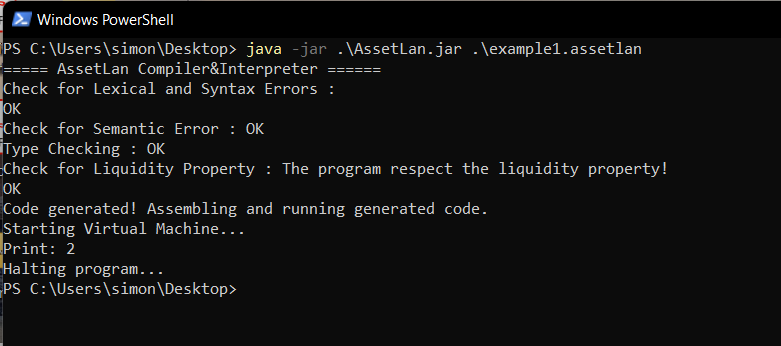
\includegraphics[width=.9\textwidth]{jarGeneration.png}
\end{figure}
Il compilatore si occupa del controllo degli errori lessicali e semantici, controllo di tipo, e se il programma rispetta la proprietà di Liquidity. Una volta eseguiti questi controlli, verrà generato un file \textit{*.asm} contenete le istruzioni che verranno prese in input dall'interprete, il quale eseguirà le istruzioni generate.

\end{document}